\begin{figure*}[t]
\centering
\begin{minipage}{.5\textwidth}
\begin{center}
\captionof{table}{\textbf{\anomalychallenge{} results:} Success rates ($\pm$ standard errors) of the evaluated models. Full results are in Appendix~\ref{app:additional_exps}.} % Overall, Gemini 2.0 Flash outperforms all evaluated models. TODO}
\label{tab:main_results_anomaly}
\begin{tabular}{lc}
\toprule
\multirow{2}{*}{Model}& \multicolumn{1}{c}{\anomalychallenge{}} \\
\cmidrule(lr){2-2}
 & Overall (\%)\\
\midrule
GPT-4o & $ 27.0 \pm 3.1 $ \\
Claude 3.5 Sonnet & $ 27.5 \pm 3.2 $ \\
Gemini 2.0 flash & $ \mathbf{35.5 \pm 3.4} $ \\
\midrule
Phi 3.5 vision & $ 0.0 \pm 0.0 $ \\
InternVL-2.5 8B MPO & $ 3.5 \pm 1.3 $ \\
Llava-Interleave-7b & $ 0.0 \pm 0.0 $ \\
Qwen2.5-VL 7B & $ 2.8 \pm 1.2 $ \\
\midrule
Qwen2-VL-72B & $ 7.5 \pm 1.9 $ \\
Llava-Onevision 72b & $ 8.5 \pm 2.0 $ \\
Pixtral-Large & $ 15.0 \pm 2.5 $ \\
\bottomrule
\end{tabular}
\end{center}
\end{minipage}%
\begin{minipage}{.5\textwidth}
\begin{scriptsize}
% \centering
\begin{center}
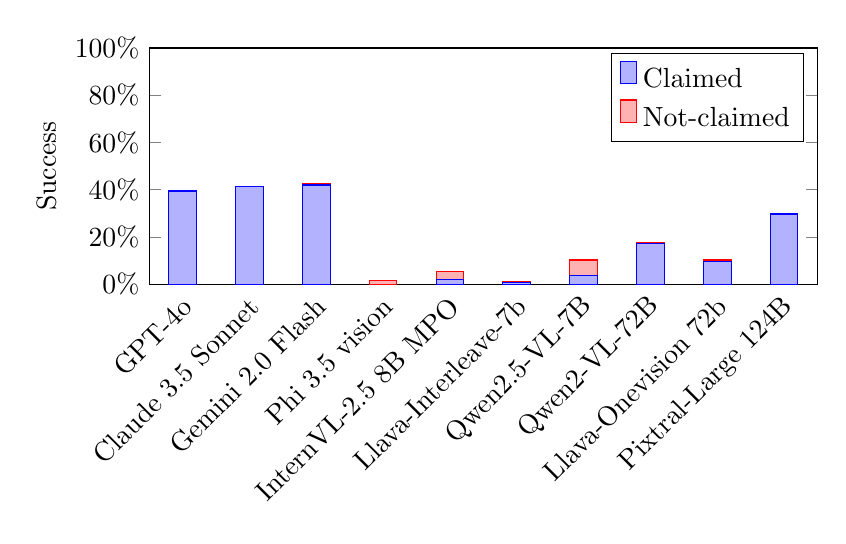
\begin{tikzpicture}
\begin{axis}[
    width=.70\linewidth,
    height=3cm,
    ybar stacked,
    yticklabel={\pgfmathprintnumber\tick\%},
    xticklabels={GPT-4o,Claude 3.5 Sonnet,Gemini 2.0 Flash,Phi 3.5 vision,InternVL-2.5 8B MPO,Llava-Interleave-7b,Qwen2.5-VL-7B,Qwen2-VL-72B,Llava-Onevision 72b,Pixtral-Large 124B},
    xticklabel style={rotate=45,anchor=east,yshift=-.2cm},
    xtick={1,2,3,4,5,6,7,8,9,10},
    xmin=0.5,
    xmax=10.5,
    ymin=0,
    ymax=100,
    x tick style={draw=none},
    scale only axis,
    % bar width=15pt,
    legend cell align={left},
    % anchor=north,legend columns=-1},
    ylabel={Success},
    ]
\addplot+[ybar] plot coordinates {(1,39.500)(2,41.250)(3,42.000)(4,0.000)(5,2.000)(6,0.750)(7,3.750)(8,17.250)(9,9.500)(10,29.750)};
\addplot+[ybar] plot coordinates {(1,0.250)(2,0.250)(3,0.750)(4,1.750)(5,3.250)(6,0.500)(7,6.500)(8,0.500)(9,0.750)(10,0.000)};
\legend{\strut Claimed, \strut Not-claimed}
\end{axis}
\end{tikzpicture}
\end{center}
\end{scriptsize}
\vspace{-1em}
\caption{\textbf{Not claimed successes in \challenge{}:} In this figure we compare the number of cases, where the agent located the object, but failed to claim the \texttt{FOUND} action. We observe, that small models often fail to format the text output to report success.}
\label{fig:nonclaim}
\end{minipage}
\end{figure*}


